%-------------------------------------------------------------------- Comente: bloquear entrada
\needspace{8\baselineskip}
\tema{Comente: ¿siempre conviene bloquear la entrada?}
\question \textbf{Comente.} En los modelos de entrada, siempre la mejor estrategia de la incumbente será bloquear la entrada.
\needspace{5\baselineskip}
\begin{solution}
Falso. La firma tiene que analizar ambas decisiones en torno a la entrada de una nueva firma al mercado. Si el beneficio de acomodar la entrada es mayor al beneficio de bloquearla, la firma incumbente decidirá acomodar la entrada. En este sentido, es muy importante que la estrategia elegida sea creíble.

\end{solution}

%-------------------------------------------------------------------- Comente: mercados desafiables
\needspace{8\baselineskip}
\tema{Comente: mercados desafiables}
\question \textbf{Comente.} La teoría de mercados desafiables nos diría que, ante pequeñas barreras de entrada, un mercado monopólico u oligopólico podría llegar a un equilibrio más similar al de competencia perfecta.
\needspace{5\baselineskip}
\begin{solution}
Verdadero. La existencia de pocas barreras de entrada genera una amenaza de competencia por parte de otras firmas, forzando a las incumbentes a comportarse de una manera más competitiva (es decir, no hay poder de mercado independiente de la concentración).

\end{solution}

%-------------------------------------------------------------------- Entrada con capacidad
\needspace{8\baselineskip}
\tema{Entrada con restricciones de capacidad}
\question Suponga que un mercado está caracterizado por la siguiente función de demanda lineal: $Q = 12 - P$. La firma incumbente ($i=1$) posee un costo marginal $c = 2$. Existe un potencial entrante ($i=2$) que posee el mismo costo marginal que la incumbente, pero si entra debe pagar un costo fijo de $F = 2$. Suponga que tanto la incumbente como el entrante poseen una restricción de capacidad de $k_i = 2$. En $t=1$ la firma entrante decide si ingresa o no al mercado; en caso de que ingrese, desembolsa $F$. Si hay entrada, en $t=2$ las firmas compiten à la Bertrand. Determine el precio, las cantidades y los beneficios de equilibrio si existiera entrada. ¿Existirá entrada en este mercado?
\needspace{5\baselineskip}
\begin{solution}
Dado que hay restricciones de capacidad, la decisión de la entrante en $t=2$ se reduce a ser \emph{demandante residual} o \emph{recortador de precios}.

\textbf{Demandante residual.} La demanda residual es la demanda descontada por la cantidad que alcance a vender la incumbente: $Q_r = 12 - 2 - P = 10 - P$. Se resuelve
\[
  \max_{P_2}\ \pi_2 = (10 - P_2)(P_2 - 2)
  \;\Rightarrow\; 10 - 2P_2 + 2 = 0
  \;\Rightarrow\; P_2 = 6, \quad Q_r = 4 .
\]
Dado que $Q_r = 4 > k_2 = 2$, la cantidad pasa a ser $2$, y el precio se ajusta para que la demanda residual sea igual a la capacidad: $10 - P_2 = 2$, es decir $P_2 = 8$. Los beneficios son $\pi_2 = (8 - 2)\cdot 2 = 12$.

\textbf{Recortar precios.} Si la entrante recorta el precio de la incumbente ($P_2 = P_1 - \epsilon$) vende toda su capacidad, con beneficios $\pi_2 = (P_1 - 2)\cdot 2$. Conviene recortar precios en lugar de ser demandante residual si $(P_1 - 2)\cdot 2 > 12$, es decir, si $P_1 > 8$. Por lo tanto, siempre que la incumbente ponga un precio mayor a 8, la firma 2 entra recortando precios, de modo que el precio de equilibrio es $P^* = 8$.

\textbf{Equilibrio.} Con $P^* = 8$, la cantidad de mercado es $Q = 12 - 8 = 4 = k_1 + k_2$: cada firma vende $q_1 = q_2 = 2$ y obtiene beneficios $\pi_1 = \pi_2 = (8-2)\cdot 2 = 12$.

\textbf{Decisión de entrada ($t=1$).} La entrante obtiene $12 - F = 12 - 2 = 10 > 0$ al entrar, y su costo de oportunidad es 0, por lo que sí habrá entrada.

\end{solution}

%-------------------------------------------------------------------- Amenazas creíbles
\needspace{8\baselineskip}
\tema{Amenazas creíbles a la entrada (capacidad)}
\question Suponga una firma incumbente que se ve enfrentada a la entrada de una nueva firma. La demanda del mercado es $P = 20 - Q$. Además, las firmas tienen costos marginales iguales a cero y tienen una capacidad fija. La firma entrante, en caso de entrar, empieza con una capacidad igual a 4. La incumbente no tiene costos de aumentar su capacidad. El precio estará dado por las capacidades ofrecidas, es decir, la cantidad será igual a la capacidad de cada firma y luego con eso se fija el precio. El juego funciona de la siguiente manera:
\begin{itemize}
  \item $t=1$: la firma entrante decide si entrar o no. En caso de no entrar, la firma entrante tiene un proyecto alternativo donde obtiene beneficios iguales a 16.
  \item $t=2$: la firma incumbente decide si actuar agresivamente o no. En caso de actuar agresivamente, elige una capacidad que minimiza las utilidades de la firma entrante. En caso de no actuar agresivamente, maximiza sus utilidades.
\end{itemize}
\begin{parts}
\part Plantee el juego y el árbol de decisión.
\needspace{5\baselineskip}
\begin{solution}
Para resolver el juego hay que calcular los pagos de las distintas alternativas.
\begin{itemize}
  \item \emph{La entrante no entra:} recibe $16$ por su proyecto alternativo y la incumbente es monopolio, con $\pi_I = 100$ ($Q = 10$, $P = 10$).
  \item \emph{La entrante ingresa y la incumbente actúa agresivamente:} la incumbente elige una capacidad que minimiza los beneficios de la entrante, es decir, que lleva el precio a cero: $P = 20 - k_I - 4 = 0$, de modo que $k_I = 16$, y ambas obtienen beneficios iguales a $0$.
  \item \emph{La entrante ingresa y la incumbente no actúa agresivamente:} la incumbente maximiza sus beneficios dado $k_E = 4$: $\max_{k_I}\ (20 - k_I - 4)k_I$, de donde $k_I = 8$, $P = 8$, $\pi_E = 8\cdot 4 = 32$ y $\pi_I = 8\cdot 8 = 64$.
\end{itemize}
\begin{center}
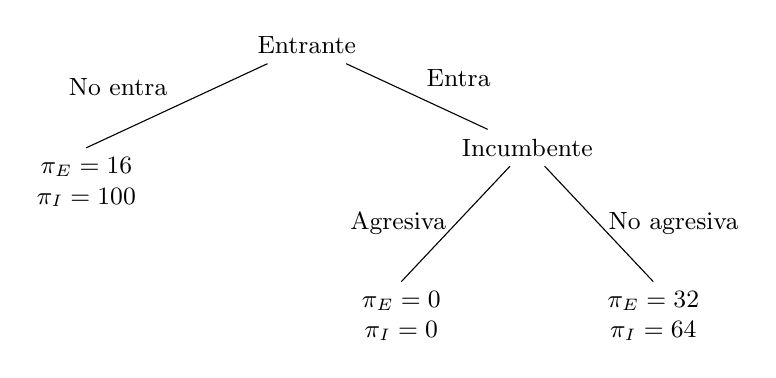
\begin{tikzpicture}[x=1cm,y=1cm,font=\small]
  \node (e) at (0,0) {Entrante};
  \draw (e) -- (-2.8,-1.3) node[midway,above left] {No entra} node[below,align=center] {$\pi_E = 16$\\$\pi_I = 100$};
  \node (i) at (2.8,-1.3) {Incumbente};
  \draw (e) -- (i) node[midway,above right] {Entra};
  \draw (i) -- (1.2,-3) node[midway,left] {Agresiva} node[below,align=center] {$\pi_E = 0$\\$\pi_I = 0$};
  \draw (i) -- (4.4,-3) node[midway,right] {No agresiva} node[below,align=center] {$\pi_E = 32$\\$\pi_I = 64$};
\end{tikzpicture}
\end{center}

\end{solution}

\part Encuentre el equilibrio y explique el resultado. ¿Qué rol juega el beneficio del proyecto alternativo de la firma entrante?
\needspace{5\baselineskip}
\begin{solution}
El equilibrio se resuelve por inducción hacia atrás. En la última etapa, la incumbente preferirá no actuar agresivamente, ya que obtiene mayores beneficios así ($64 > 0$). Sabiendo esto, la firma entrante preferirá ingresar al mercado, ya que la competencia no agresiva le reporta un beneficio mayor que su proyecto alternativo ($32 > 16$). A la incumbente le gustaría amenazar con actuar agresivamente para evitar la entrada y obtener un beneficio de $\pi_I = 100$, pero no puede hacer esta amenaza creíble. La razón es que, una vez que se produce la entrada, actuar agresivamente no es la mejor opción para la incumbente.

El beneficio del proyecto alternativo de la entrante ($16$) representa el costo de oportunidad de la firma al decidir entrar o no: si la firma entra y obtiene beneficios nulos, habría perdido el beneficio alternativo de 16.

\end{solution}

\part Suponga ahora que la firma incumbente puede elegir su capacidad antes de la entrada. ¿Cuál será la mejor opción de la incumbente en este caso?
\needspace{5\baselineskip}
\begin{solution}
En este caso la incumbente puede fijar una capacidad para desincentivar la entrada de la competencia. Sin embargo, esta estrategia solo es conveniente si los beneficios son mayores que permitir la entrada, lo que anteriormente generaba una utilidad de $\pi_I = 64$. El nivel de capacidad que desincentiva la entrada es tal que los beneficios de la entrante sean menores que su proyecto alternativo:
\[
  \pi_E = (20 - k_I - 4)\cdot 4 < 16 \quad\Longrightarrow\quad k_I > 12 .
\]
Por lo tanto, la incumbente debe fijar una capacidad de al menos 13 unidades. Si lo hace, los beneficios serán los monopólicos menos los costos de inversión en capacidad (la pauta supone un costo de $3$ por unidad de capacidad):
\[
  \pi_I = 100 - 3\cdot 13 = 61 .
\]
Dado que estos beneficios son menores que $\pi_I = 64$, la mejor opción de la incumbente será permitir la entrada y escoger su capacidad posterior para maximizar sus beneficios.

\end{solution}
\end{parts}

%-------------------------------------------------------------------- Demasiadas empresas
\needspace{8\baselineskip}
\tema{¿Demasiadas empresas en la industria? (costos fijos y Cournot)}
\question \textbf{Comente.} Mientras más empresas haya en una industria más eficiente será, puesto que un número reducido de estas podría llevar a mayor poder de mercado reduciendo el bienestar de los consumidores. Verdadero o falso.
\needspace{5\baselineskip}
\begin{solution}
Depende. Si bien la intuición es correcta, dado que a mayor cantidad de empresas podría reducirse el índice de Lerner (y con ello el poder de mercado), en la realidad hay fricciones que considerar. En gran parte de las industrias los costos fijos (de entrada o recurrentes) que enfrenta cada firma son considerables: mientras más firmas haya, más costos fijos se pagarán, lo cual impacta negativamente la eficiencia (estática). En la misma línea, la presencia de economías de escala debería presionar a la baja los precios. Por lo tanto hay un \emph{trade-off} entre la competencia dada por la cantidad de firmas y la ineficiencia debida a costos fijos y economías de escala.

\end{solution}

%-------------------------------------------------------------------- Cournot con costo fijo
\needspace{8\baselineskip}
\tema{Número de firmas en Cournot con costo fijo y bienestar}
\question Considérese una industria homogénea con $N$ empresas perfectamente simétricas. Las empresas deciden de forma simultánea la cantidad que llevarán al mercado, y tienen un costo de producción $C = cq + F$, donde $c$ es el costo marginal y $F$ un costo fijo. La demanda del mercado se caracteriza por $P = 1 - Q$, siendo $P$ el precio de mercado y $Q$ la producción total.
\begin{parts}
\part Plantee la maximización de beneficios de una empresa $i$ que elige $q_i$.
\needspace{5\baselineskip}
\begin{solution}
\[
  \max_{q_i}\ \pi_i = \Bigl(1 - q_i - \sum_{j\neq i}q_j\Bigr)q_i - cq_i - F .
\]

\end{solution}

\part Derive las condiciones de primer orden e imponga la simetría para llegar a la cantidad de equilibrio.
\needspace{5\baselineskip}
\begin{solution}
La CPO es $1 - 2q_i - \sum_{j\neq i}q_j - c = 0$, es decir, $q_i = \frac{1 - c - \sum_{j\neq i}q_j}{2}$. Imponiendo $q_i = q_j = q^*$:
\[
  q^* = \frac{1 - c}{N + 1}.
\]

\end{solution}

\part Encuentre, con la cantidad de equilibrio, el precio de equilibrio, el cual debe depender del número de firmas en el mercado. ¿Qué efecto tiene $N$ sobre $P$ y sobre el excedente del consumidor?
\needspace{5\baselineskip}
\begin{solution}
$Q^* = Nq^* = \frac{N(1-c)}{N+1}$, de modo que
\[
  P^* = 1 - \frac{N(1-c)}{N+1} = \frac{1 + Nc}{N+1}.
\]
A mayor $N$, menor $P^*$ y mayor es el excedente de los consumidores.

\end{solution}

\part ¿Cuál es el efecto de un mayor $N$ sobre los beneficios de las empresas y el excedente de los productores?
\needspace{5\baselineskip}
\begin{solution}
Los beneficios de cada firma, incluyendo el costo fijo, son
\[
  \pi_i = (P^* - c)q^* - F = \frac{(1-c)^2}{(N+1)^2} - F ,
\]
que son decrecientes en $N$. El excedente de los productores (suma de los beneficios de las $N$ empresas) es
\[
  EP = \frac{N(1-c)^2}{(N+1)^2} - NF .
\]

\end{solution}

\part ¿Qué ocurre con el excedente del productor encontrado cuando $N$ aumenta?
\needspace{5\baselineskip}
\begin{solution}
El excedente del productor de la industria disminuye con $N$ (el primer término decrece a partir de $N = 1$ y el segundo término, $-NF$, decrece linealmente). Observe que a medida que $N$ aumenta y finalmente tiende a infinito, el excedente del productor y el bienestar total pueden volverse negativos: si bien el excedente del consumidor aumenta, el costo fijo total $NF$ crece sin límite y el bienestar total tiende a $-\infty$. De ahí la idea de que puede haber demasiadas empresas en una industria.

\end{solution}
\end{parts}

%-------------------------------------------------------------------- Comente: N exógeno
\needspace{8\baselineskip}
\tema{Comente: número de empresas exógeno en modelos de entrada}
\question \textbf{Comente.} En los modelos de entrada, el número de empresas es exógeno y no depende de las condiciones del mercado.
\needspace{5\baselineskip}
\begin{solution}
Falso. En los modelos de entrada el número de empresas depende del tipo de competencia, de los costos fijos y marginales; por lo tanto, la cantidad de firmas es endógena.

\end{solution}

%-------------------------------------------------------------------- Comente: condición de equilibrio de N
\needspace{8\baselineskip}
\tema{Comente: condición de equilibrio del número de firmas}
\question \textbf{Comente.} La condición para que un número $N$ de empresas esté en equilibrio es que las ganancias sean no negativas para esas empresas, pero negativas si entra una empresa adicional.
\needspace{5\baselineskip}
\begin{solution}
Verdadero. El equilibrio de Nash para la cantidad de firmas se da en el punto en que $\pi^*(N) \geq 0$ y $\pi^*(N+1) < 0$: la entrada de una nueva firma le implicaría utilidades negativas.

\end{solution}

%-------------------------------------------------------------------- Comente: Bertrand con costos fijos
\needspace{8\baselineskip}
\tema{Comente: Bertrand con costos fijos positivos}
\question \textbf{Comente.} En competencia à la Bertrand con costos fijos positivos, el equilibrio suele implicar múltiples empresas compitiendo en precios.
\needspace{5\baselineskip}
\begin{solution}
Falso. En Bertrand con costos marginales simétricos el precio llegaría al costo marginal y los beneficios serían cero. Dados costos fijos positivos, entonces ninguna firma obtiene utilidades no negativas si hay dos o más firmas. \emph{Nota:} solo habrá una firma, que cobra más que el costo marginal pero no el precio que pondría un monopolista normal. Si cobra el precio de monopolio podría atraer la entrada, por lo que, siguiendo la idea de mercados desafiables, la firma cobrará el costo medio.

\end{solution}

%-------------------------------------------------------------------- Comente: diferenciación y entrada
\needspace{8\baselineskip}
\tema{Comente: bienes muy diferenciados y entrada}
\question \textbf{Comente.} Si los bienes están muy diferenciados, la entrada de nuevas empresas puede generar un mayor bienestar social.
\needspace{5\baselineskip}
\begin{solution}
Verdadero. Productos muy diferenciados tienen valor agregado y el \emph{business stealing} es más difícil. La entrada de nuevas firmas implica una mayor variedad para los consumidores, generando mayor excedente del consumidor. Además, mayor competencia induce a menores precios y por tanto mayor excedente del consumidor.

\end{solution}

%-------------------------------------------------------------------- Comente: Sutton
\needspace{8\baselineskip}
\tema{Comente: costos endógenos de entrada (Sutton)}
\question \textbf{Comente.} Según el modelo de Sutton, mayores costos endógenos de entrada están asociados con menor concentración en la industria y por tanto menos competencia.
\needspace{5\baselineskip}
\begin{solution}
Falso. Los costos endógenos tienen un factor estratégico que tiende a concentrar la industria. Un ejemplo de industria con altos costos de entrada endógenos es el \emph{retail}: la publicidad es un factor estratégico que deciden las firmas y que detiene a posibles firmas entrantes de ingresar al mercado. Este es un mercado que, a pesar de estar concentrado, tiene un nivel de competitividad alto.

\end{solution}

%-------------------------------------------------------------------- Comente: mercados desafiables y economías de escala
\needspace{8\baselineskip}
\tema{Comente: mercados desafiables y economías de escala}
\question \textbf{Comente.} El modelo de mercado desafiable contradice la idea de que las economías de escala necesariamente implican poder de mercado.
\needspace{5\baselineskip}
\begin{solution}
Verdadero. Baumol demuestra que las economías de escala no implican poder de mercado si el mercado es desafiable. La amenaza creíble de entrada puede mantener los precios competitivos incluso con un solo productor. \emph{Nota:} si se aprovecha la economía de escala entonces el precio bajaría, pero eso no implica que la amenaza de entrada sea menos creíble.

\end{solution}

%-------------------------------------------------------------------- Comente: entrada de firma eficiente
\needspace{8\baselineskip}
\tema{Comente: entrada de una firma muy eficiente y concentración}
\question \textbf{Comente.} El mercado de la atrapada de dos se compone de firmas simétricas que compiten à la Cournot y enfrentan una demanda lineal. El pasado cuatrimestre irrumpió una nueva firma mucho más eficiente. El mercado ahora está más concentrado y el precio es menor. ¿Cómo se explicaría esta aparente contradicción?
\needspace{5\baselineskip}
\begin{solution}
Si la empresa entrante es mucho más eficiente, el precio tiende a la baja. Por otro lado, se rompe la simetría: para todas las firmas antiguas los beneficios se verán reducidos, puesto que con Cournot asimétrico la firma más eficiente acapara más mercado. Esta reducción de beneficios podría llevar a un menor número de firmas. Por lo tanto, el precio sería menor pero con una mayor concentración de mercado (concentración y competencia no se mueven necesariamente en direcciones opuestas).

\end{solution}

%-------------------------------------------------------------------- Costos de entrada exógenos y tamaño del mercado
\needspace{8\baselineskip}
\tema{Costos de entrada exógenos, tamaño de mercado y concentración}
\question Note que cuando hablamos de costos de entrada no nos referimos exactamente a lo mismo que costos fijos. Explique cómo se relacionan el tamaño del mercado y la concentración (1/$N$) bajo costos de entrada exógenos, distinguiendo entre competencia à la Bertrand y à la Cournot.
\needspace{5\baselineskip}
\begin{solution}
Bajo Bertrand, la cantidad de firmas será siempre una: una firma adicional bajo Bertrand implicaría llevar el precio a un nivel no sostenible (utilidades negativas). En Bertrand con costos fijos, la entrada de una nueva firma solo es posible si logra tener un costo medio más bajo que el de la incumbente; si entra una más eficiente, la incumbente sale del mercado. La concentración no baja con el tamaño del mercado.

En el caso de Cournot, la concentración de mercado disminuye mientras más grande sea el mercado. Pero esto no es una relación 1:1, ya que los costos fijos hacen que el tamaño de mercado tenga un menor efecto sobre la cantidad de firmas. Por ejemplo: si aumenta la población, aumenta la demanda por peluquerías y por aeropuertos; si aumenta el número de peluquerías en 500 nuevos locales, sería absurdo pensar que ahora habrá 500 nuevos aeropuertos. Sujeto a estar en un cartel, los beneficios serán mayores dada la menor competencia, lo que atrae más entrada y menor $1/N$. El gráfico (concentración vs.\ tamaño de mercado) muestra que mayores niveles de competencia podrían estar relacionados a menores niveles de concentración.

\end{solution}

%-------------------------------------------------------------------- Derivación N Cournot
\needspace{8\baselineskip}
\tema{Derivación del número de firmas en Cournot con demanda lineal}
\question Los modelos de entrada piensan la entrada de $N$ firmas como un equilibrio de Nash que cumple: (1) $\pi^*(N) \geq 0$ y (2) $\pi^*(N+1) < 0$. Para caracterizar esta condición es necesario plantear un tipo de competencia y una función de demanda. La demanda del mercado es $Q = S\,q_d$, donde $S$ es el tamaño de mercado y $q_d = a - bP$ la cantidad demandada per cápita. La función de costos es $C_i(q_i) = cq_i + F$, con $c$ el costo marginal y $F$ un costo fijo.
\begin{parts}
\part Llegue a la cantidad producida por cada empresa bajo competencia por cantidades. \emph{(Indicación: llegue a la demanda inversa y defina $\alpha = a/b$, $\beta = 1/(Sb)$.)}
\needspace{5\baselineskip}
\begin{solution}
Despejando, $P = \frac{a}{b} - \frac{Q}{Sb} = \alpha - \beta Q$. Con $N$ firmas, cada una maximiza $q_i\bigl(\alpha - \beta\sum_j q_j - c\bigr) - F$, con CPO $\alpha - c - \beta\sum_{j\neq i}q_j - 2\beta q_i = 0$. Por simetría,
\[
  q^* = \frac{\alpha - c}{(1+N)\beta} = S\,\frac{a - bc}{1+N}.
\]

\end{solution}

\part Dada la cantidad de Cournot, encuentre la función de utilidades de la firma. \emph{(Indicación: exprese primero $Q$ y luego úselo para expresar $P(Q) - c$ y sustitúyalo en $\pi_i$.)}
\needspace{5\baselineskip}
\begin{solution}
La cantidad total es $Q^* = \frac{NS(a - bc)}{1+N}$, de modo que $P(Q^*) = \alpha - \beta Q^* = \frac{a}{b} - \frac{N(a-bc)}{b(1+N)}$ y
\[
  P(Q^*) - c = \frac{a - bc}{b(1+N)}, \qquad
  \pi^*(N) = \bigl(P(Q^*) - c\bigr)q^* - F = \frac{S(a - bc)^2}{b(1+N)^2} - F .
\]

\end{solution}

\part Encuentre el número de firmas del mercado dada la condición de entrada. ¿Qué tan elástica es la cantidad de firmas al tamaño de mercado?
\needspace{5\baselineskip}
\begin{solution}
La condición de entrada es $\pi^*(N) \geq 0$, es decir,
\[
  \frac{S(a-bc)^2}{b(1+N)^2} \geq F
  \quad\Longleftrightarrow\quad
  N^* = (a - bc)\sqrt{\frac{S}{bF}} - 1 .
\]
$N^*$ es creciente en el tamaño de mercado $S$, pero la elasticidad es menor a 1: un aumento de 1\% del mercado se traduce en menos de 1\% más de firmas (en efecto, $\varepsilon_{N,S} = \frac{1}{2}\frac{N^*+1}{N^*} < 1$ para $N^* > 1$).

\end{solution}

\part ¿Qué representa $b$? ¿Cuál es su efecto en el número de firmas? Justifique.
\needspace{5\baselineskip}
\begin{solution}
$b$ es la sensibilidad de la demanda per cápita al precio (cuánto cae la cantidad demandada cuando sube el precio), es decir, la pendiente de la demanda y, por lo tanto, mide cuán elástica es. $\frac{\partial N^*}{\partial b} < 0$: a mayor sensibilidad al precio, el margen de las firmas es menor, los beneficios caen y entran menos firmas.

\end{solution}
\end{parts}
